\chapter{Introduction} \label{chapter:intro}
\section{Problem}
Ordnance Survey (OS) is a government-owned national mapping agency for Great Britain. As a company, they take great pride in producing high-quality maps, both digital and in sheet-form, using high-resolution aerial photographs (up to 1 pixel per 25$\times$25cm) taken by a 196-megapixel camera from a plane flying at 3000 ft \citep{nelson_2014} (see figure \ref{fig:aerial}).

\begin{figure}[H]
    \centering
    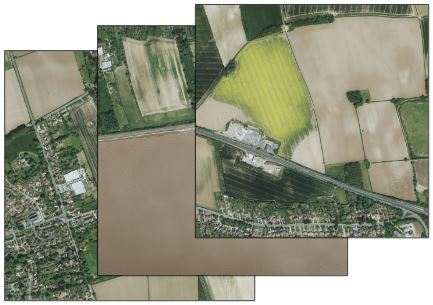
\includegraphics{figs/1/aerial}
    \caption{OS Aerial Images}
    \label{fig:aerial}
\end{figure}

Their flagship product is OS MasterMap, a database that contains information regarding every feature in Great Britain visible from aerial imagery, displayed on a continuous digital map (see figure \ref{fig:mastermap})

\begin{figure}[H]
    \centering
    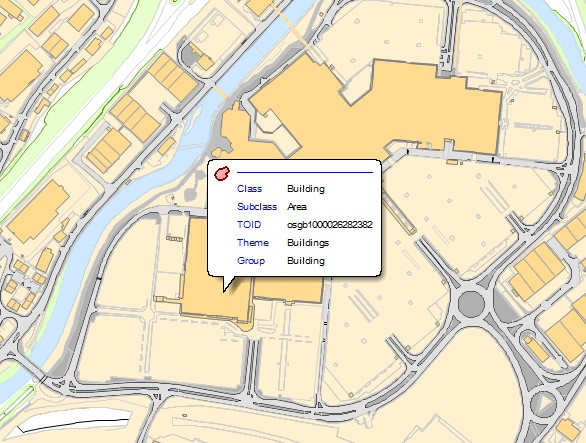
\includegraphics[width=\textwidth]{figs/1/mastermap}
    \caption{OS MasterMap Example}
    \label{fig:mastermap}
\end{figure}

\section{Solution}
OS believe it is possible to automate this process using transfer learning, and have introduced their idea, ``The Productizer'' (see appendix \ref{appendix_proposal}). 
The Productizer will use machine learning to automatically identify features in an aerial image by scanning the image and extracting a hierarchy of attributes from each potential feature. Patterns in these attributes can be used to identify the specific feature, much like a fingerprint. The user will train the tool with supervised data to generate a mapping between the attribute fingerprints and their corresponding feature. 
Using transfer learning, the tool will then scan the rest of the image to find sections that match this fingerprint, thus finding additional occurrences of the feature. The tool would require an easy-to-use interface to hide the complexity of the system, allowing users with no machine-learning experience to train the classifier and obtain its predictions.

\section{Goals}
The goals of the system are as follows:
\subsection{Functional}
\begin{itemize}
    \item Accepts uploading of any Ordnance Survey aerial image
    \item Enables the selection of any feature on the image
    \item Extracts information from selected features that can be used by classification algorithms to identify that feature, much like a fingerprint
    \item Classifier can be trained to identify features using extracted information 
    \item Provides an intuitive interface to easily train the classifier and obtain its predictions, hiding the complexity of the program from the user
    \item Supports iterative training over a dynamic number of classes
    \item Developed as a cloud-based application, usable by multiple users concurrently
\end{itemize}
\subsection{Non-Functional}
\begin{itemize}
    \item Capable of classifying features with an accuracy of 80\%+
    \item Capable of classifying features into 100 separate classes
    \item Processing time for each tile is less than 0.1s
    \item Sufficient supervised training data can be gathered by the user within 5 minutes per class
    \item When used by an expert, results in increased levels of productivity compared to manual identification
\end{itemize}
\subsection{Stretch}
\begin{itemize}
    \item Uses microservices to run separate modules concurrently
    \item Uses contextual information gathered from surrounding tiles to classify tiles
    \item Enables re-training of classifier when it incorrectly classifies a feature
    \item Supports deletion of unfavourable training data
\end{itemize}



